\documentclass[12pt]{dissertation} 

%load any additional packages
\usepackage{amssymb}
\usepackage{natbib}
\title{Differential IP clustering for Vulnerability Detection using applied Machine Learning} 
\author{Sebastian Bocquier}             %your name
\college{Division of Computing and Mathematics}  %your college

%\renewcommand{\submittedtext}{change the default text here if needed}
\degree{Honours of Science \\in\\ Ethical Hacking and Computer Security}     %the degree
\degreedate{\small \textit{\today}}         %the degree date

%end the preamble and start the document
\begin{document}

%this baselineskip gives sufficient line spacing for an examiner to easily
%markup the thesis with comments
\baselineskip=18pt plus1pt

%set the number of sectioning levels that get number and appear in the contents
\setcounter{secnumdepth}{3}
\setcounter{tocdepth}{3}


\maketitle                  % create a title page from the preamble info
% !TEX root = dissertationmain.tex
\begin{dedication}
This thesis is dedicated to\\
 no one\\
for no special reason\\
\end{dedication}        % include a dedication.tex file
% !TEX root = dissertationmain.tex
\begin{acknowledgements}
I would like to take this opportunity to thank my project supervisor, Xavier Bellekens, who introduced me to the topic of Machine Learning and offered guidance from the beginning through to the completion of this project. Without whom this project would not have been possible. I would also like to thank the module leader, Colin McLean, who has given me continuous advice throughout my years of study at Abertay University.
\end{acknowledgements}   % include an acknowledgements.tex file
% !TEX root=dissertationmain.tex
\begin{abstractlong}
The field of computing and networking security has had much research and innovation in applied machine learning within software tools. However, this focus has primarily been on blue team, leaving the red team behind and lacking in innovation. The nature of red teaming requires advanced tools to counter the increasing complexity of those used by blue team. Therefore, if a balance in research and innovation is not retained, red teaming will risk becoming obsolete. Related literature has been reviewed to provide a basis of understanding in the subject area.

The purpose of this thesis is to create a proof of concept tool which will aid in red teaming activities using machine learning techniques, as well as create grounds for further research into the field. The application created is able to determine the highest probable, vulnerable hosts in a network, as well as return full clusterings of the network for each form of input. The application has several different modes which require at least one file input from common network scanning tools in order to function. The application determines these vulnerable hosts by using several different clustering and statistical calculations with a small bias towards vulnerability data. The results are displayed in text form with varying levels of verbosity. There is an optional GUI to display the results in greater detail, which includes manipulatable clustering graphs and host information. The application is highly configurable, portable and versatile, allowing it to be used on any size or type of network topology. 

The application was tested on a network dataset consisting of approximately fifty hosts and was found to have successfully determined the vulnerable hosts and achieved the initial design goals it was set. The application was critically reviewed in depth, and was found that it had an issue in determining vulnerable hosts on a network, in which the majority of hosts are vulnerable. In this scenario, the application will disregard the vulnerabilities of those hosts as it deems them to be insufficiently different. Unfortunately, due to the sensitive nature of the datasets required and project time constraints, only one network dataset was used. This issue is due to the application's core design; several solutions, as well as improvements of varying complexity are provided as future development recommendations. 

The positive results of the thesis show that red teaming is able to benefit from applied machine learning techniques and that more research needs to be conducted in this field.
\end{abstractlong}          % include the abstract

\begin{romanpages}          % start roman page numbering
\tableofcontents            % generate and include a table of contents
\listoffigures              % generate and include a list of figures
\end{romanpages}            % end roman page numbering

%now include the files of latex for each of the chapters etc
% !TEX root = dissertationmain.tex
%Chapter
\chapter{Introduction}
\label{chap:chapter1}


\paragraph{}This section will give a brief background and history of Machine Learning before going in to depth with the definitions and types of algorithms used in modern Machine Learning systems. An analyses of the impact Machine Learning has in the field of computer security and how it can be applied directly to penetration testing and red teaming. Research aims and objectives will be provided as well as a statement to the structure of the rest entire thesis.



%Section
\section{Background}
\label{sec:section1}

\paragraph{}The term machine learning was first defined by Arthur Samuel in the year 1959 as a "Field of study that gives computers the ability to learn without being explicitly programmed" and later as "a field of study that concentrates on induction algorithms and on other algorithms that can be said to 'learn'", \cite{ronKohavi}. Machine learning has largely evolved from several subfields of artificial intelligence, specifically, computational learning and pattern recognition but now it stands on its own with its subfield Deep Learning being at the forefront of technology. Machine learning consists of the studying and construction of algorithms that can learn from and make predictions of data, \cite{bigData}. The early information available for machine learning was almost entirely theoretical due to the lack of processing power at the time. One of the early pioneers was \cite{Valiant} whom developed a PAC learning framework and established the theory of a learnable algorithm, \cite{mlOpt}.  Modern machine learning algorithms use many calculations from statistics, information theory, theory of algorithms, probability and functional analyses, \cite{mlOpt}.

%Section
\section{Current state of Machine Learning}
\label{sec:section2}


\paragraph{}In the recent year’s, machine learning accuracy and efficiency has increased dramatically which has caused the field to rapidly gain in popularity, especially in deep learning. One of the major reasons for this is due to the improvement in graphics processing units which in some computational tasks can outperform central processing units by an order of magnitude or more, \cite{CNNperf}. The rapidly growing field of deep learning could be made apparent by Google’s recent self-driving car and LeNet image recognition system, however, examples of machine learning can be found in just about every field with a classification or regression problem. Some of which include: natural language processing using morphological analyses for linguistics (\cite{NLP}), document classification and spam detection, better image recognition than humans (\cite{manualclassifying}) and beating a professional player at the complex Chinese game ‘Go’ (\cite{Gobot}). Figure ~\ref{fig:aitimeline} illustrates the advancement of machine learning using the context of game artificial intelligence players.

%Figure
\begin{figure} 
   \centering
   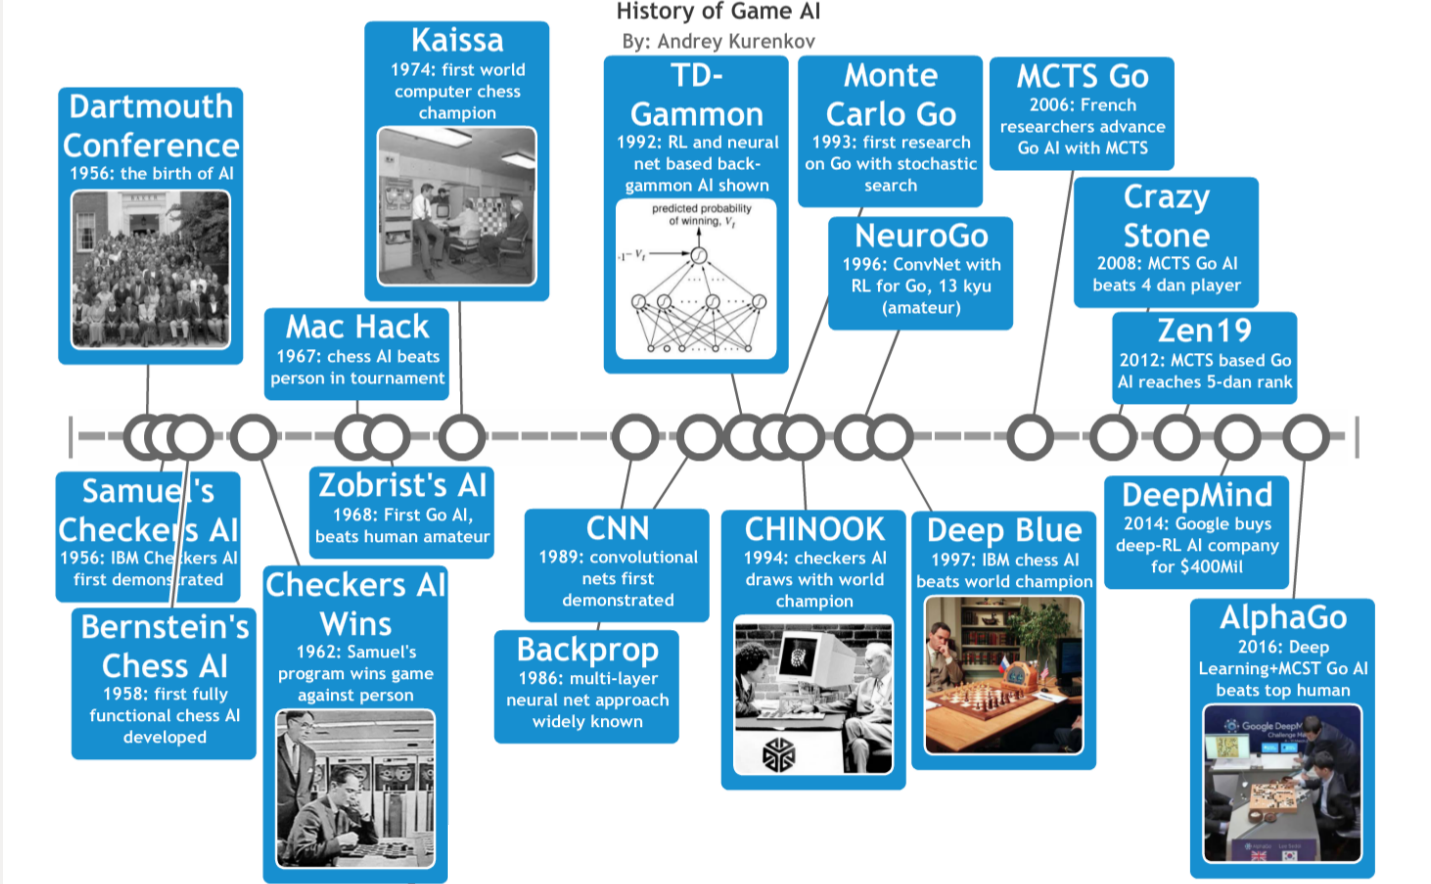
\includegraphics[width=0.95\textwidth]{Figures/aitimeline.png}
   \caption[Timeline of artificial intelligence for games]{ Timeline of artificial intelligence for games, ~\cite{timeline}}
   \label{fig:aitimeline}
\end{figure}


\paragraph{}The majority of projects over the past few years have focused on Deep Learning due to its performance and versatility with complex problems but also because of the media coverage with large scale projects by international corporations such as Google and Microsoft. The idea of deep learning has been around since the 1980’s where a Japanese scientist, Kunihiko Fukushima, proposed a hierarchical, multi-layered artificial neural network named Neocognitron, designed for handwritten character recognition. Neocognitron was recognised as the inspiration for convolutional neural networks, the most commonly used deep learning algorithm, \cite{DeepLearning}.  Deep learning attempts to model complex abstractions in data by using a multiple-level architecture most commonly compromising of artificial neural networks and non-linear transformations in its algorithms, \cite{CNNperf}.  As such, the concepts of deep learning are extensions of regular machine learning algorithms.
\paragraph{}In the past year a new topic has become of consider interest in the machine learning field, Automated Machine Learning, which can be considered to cover the tasks of algorithm selection, hyperparameter tuning, iterative modelling and model assessment, \cite{autoML}. By the end of 2016 the python Auto-sklearn library was created based off of the scikit-learn library which encompasses these tasks, created by a team from the University of Freiburg it won the KDnuggets AutoML challenge, \cite{auto-skl}. Using these examples, it’s possible to hypothesize that the future of machine learning will include automatic deep learning, however, these individual fields of machine learning are still in their infancy and far from being used together.
\paragraph{}The computer security industry due to its nature, has many examples of machine learning implementations such as intrusion detection systems using machine learning or deep learning for anomaly detection. One of which has been commercialised under the company name ‘Deep Instinct’ and advertises zero-day detection using deep learning. However, the majority are very similar and are all blue team based security solutions. Researching into Red team or penetration testing tools using machine learning resulted in a disappointing lack of tools or ideas considering the vast amount available for Blue team. 
\paragraph{}The sole documented research found for red team was for an automatic penetration testing project named Auto Red Team (ART) framework by Lu, Song of Iowa State University in 2008 which used decision trees and hard programmed exploits. This meant the entire hard programmed exploit section had to be reconstructed for each use case, this would not be ideal but also extremely time consuming. Further analyses of the ART framework can be found in the literature review of "Auto Red Team: a network attack automation framework based on decision tree". There have also been tools and libraries created to test the security of software which use machine learning models such as Deep Pwning. Deep Pwning is an open source metasploit plugin which allows the tricking of machine learning models. This field of research was named Adversarial Machine learning and the first paper of which was respectably named "Adversarial Machine Learning" and published by ACM in 2011.
\paragraph{}There is an extensive amount branches to machine learning and unfortunately, too many to cover in this thesis due to time constraints. Therefore, this introduction will only detail the most popular types of machines learning algorithms.


%Section
\section{Significance of study}
\label{sec:section3}


\paragraph{}The increased demand for penetration testers justifies the need for more effective and advanced tools to conduct their security assessments. The goal of a penetration test being to find vulnerabilities in a system using techniques similar to that of a malicious hacker. This means malicious hackers will continue to use the most advanced methods to gain access to critical systems and thus security teams must also continue to advance their toolset to be as effective and efficient as possible. Penetration tests can last a time scale of anything between one day to several months and more advanced machine learning tools would allow for a more efficient use of this time. The large variety of machine learning models used in the blue team results in a large variety of models required to test them using adversarial machine learning as well as advanced machine learning tools, specifically for the red team in order to bring each team to the same level. Having both red team and blue team on the same level is beneficial for the industry as a whole, providing competition between both sides and to continue to strive for improvement. This project aims to help correct this balance by creating a useful red team tool using machine learning.


%Section
\section{Types of Machine learning}
\label{sec:section4}

\paragraph{}As mentioned above there are many different machine learning algorithms available. Each algorithm can be classed based on the problem, required output and several factors of the data set, such as whether it includes labels and the amount of values it includes. The two primary problems machine learning algorithms provide solutions to, can be put in to two categories which are not mutually exclusive and can be combined in certain use cases. These are classification and regression problems. The following describes and states the differences of these types.


\subsection{Classification} 
\label{ssec:subsection1}

\paragraph{}With the growth of big data, unstructured data is more prevalent than its structured counterpart. This is because, "while the amount of structured data has grown fast, the amount of unstructured data has grown much faster" \cite{bigData}. This creates the need for ever more efficient data analytics and is a typical classification problem for machine learning. There are many types of classification, simple types such as a linear classifier and then more complex types such as multiclass and structured classifiers. Classification is largely used in data mining and statistical analyses for these purposes. In short, classification is used when you require an input variable to be identified as part of a group or label, resulting in the full dataset being categorised. Classification can only take a finite set of values such as picking from 1 of N values. In classification, each incorrect answer is equally incorrect, compared to regression where incorrect answer can be varying levels of incorrect.

\subsection{Regression} 
\label{ssec:subsection2}

\paragraph{}Regression problems are for when prediction of real continuous values is required, such as predicting stock market values and detecting the age of a person from a picture, \cite{pythonML}. Regression analyses involves predicting and estimating a response based on previous data and input variables. As mentioned above regression answers can have a varying level of inaccuracy as appose to binary correct or false predictions. This is due to regression using continuous values.
Figure ~\ref{fig:regvsclass}  provides a basic illustration example of these two problems.

%Figure
\begin{figure} 
   \centering
   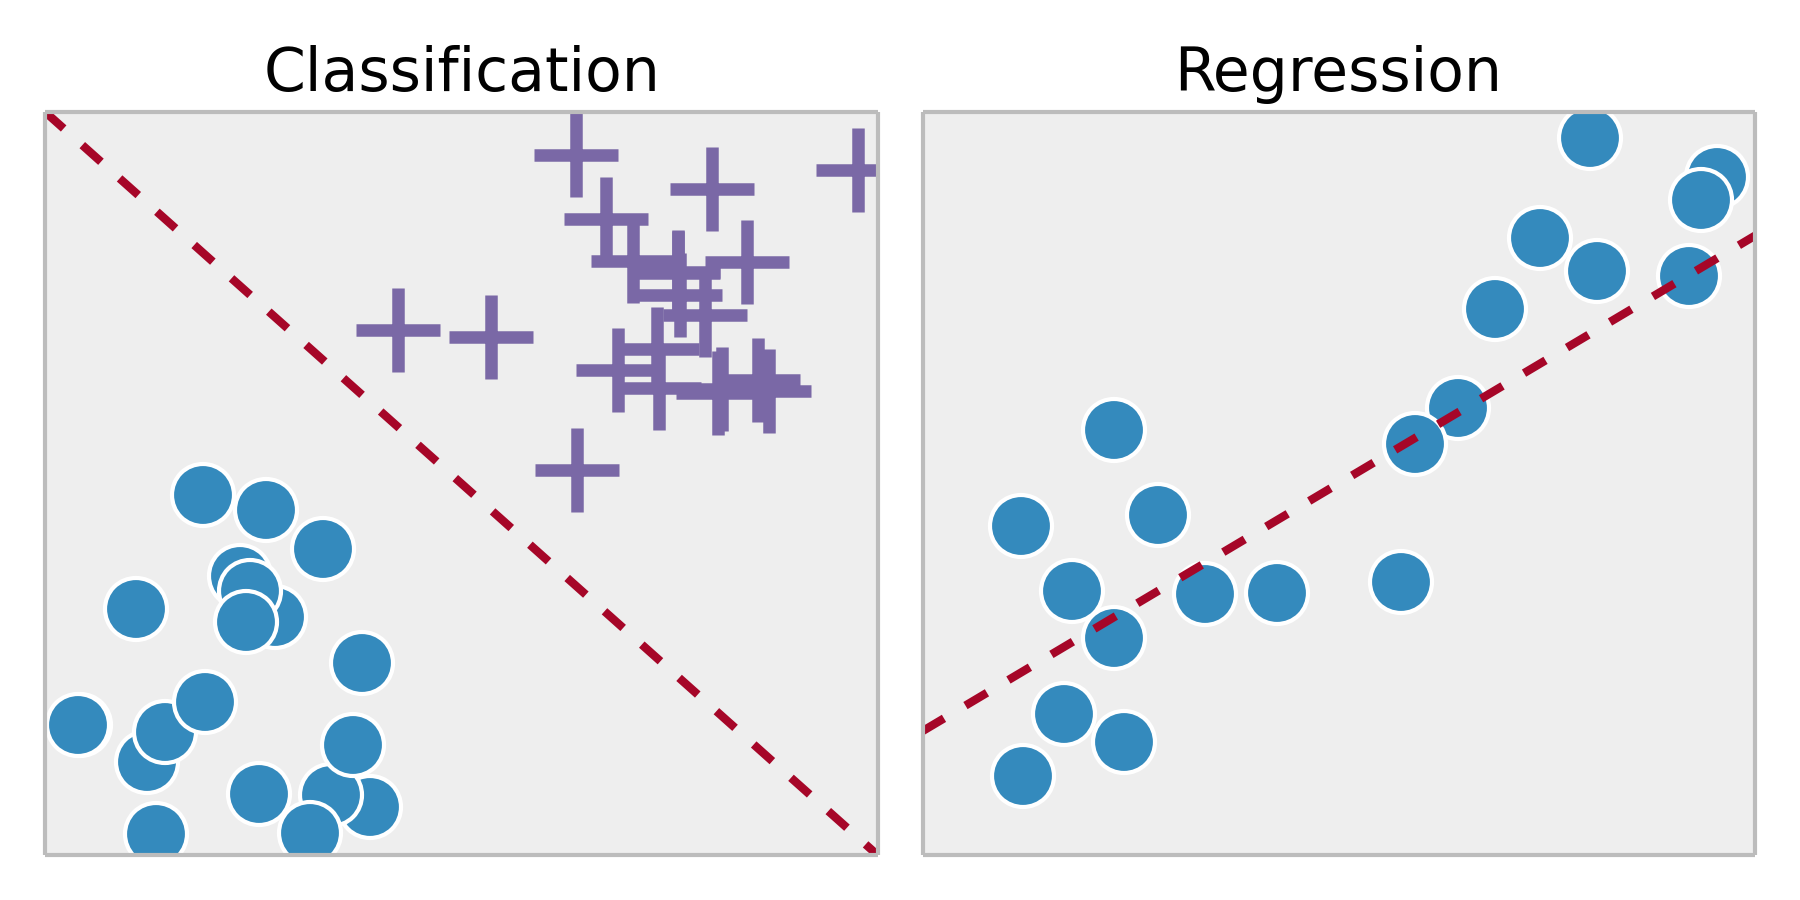
\includegraphics[width=0.95\textwidth]{Figures/ml.png}
   \caption[Illustration of machine learning types]{ Illustration of machine learning types, ~\cite{pythonML}}
   \label{fig:regvsclass}
\end{figure}


%Section
\section{Types of Learning algorithms}
\label{sec:section5}

\paragraph{}The most commonly found learning methods for algorithms are supervised and unsupervised followed by semi supervised and reinforcement learning which are also fairy common. These are explained briefly as follows.

\subsection{Supervised}
\label{ssec:subsection3}

\paragraph{}In a supervised training model, the entire data-set used for training is pre-labelled so that the algorithm can use pattern analyses to predict given values after training. A use case scenario for supervised learning includes the above stock market example where current values with labels are given and the model is used to predict future labels.

\subsection{Semisupervised} 

\label{ssec:subsection4}

\paragraph{}Due to the expensive nature of labelled data in most cases, semisupervised learning uses a split of labelled and unlabelled data to train the model. This is most often split unevenly with the large majority of training data being unlabelled. This model is often used in cases where the cost of labelled data-sets is simply too expensive.

\subsection{Unsupervised} 

\label{ssec:subsection5}

\paragraph{}The opposite of supervised learning, where the training data-set has no labels and the model must attempt to determine the correct answer itself. This is often used as a method to determine a structure in the data given. These models can identify segments of similar attributes such as clustering. Unsupervised learning is the primary method used for this thesis’s methodology.

\subsection{Reinforcement} 
\label{ssec:subsection6}
\paragraph{}Reinforcement learning works similarly to heuristic algorithms in the sense that every possibility is attempted and assigned a score in which the iteration with the highest score is used as the model output. Whilst training this model the algorithm uses the highest score’s iteration to modify its calculations for greater accuracy and efficiency. This model is often used in robotics as well as game design for path navigation calculation and computer player AI (artificial intelligence). The following is an example use case: A chess player AI calculates each possible move it can make using a reinforcement model for each of its turns. The model assigns a score to each move it could possible make at that point in time and weights them based on pieces acquired, future strategy prospects and defence risk.
Similar models have been used for AI’s mentioned in Figure ~\ref{fig:aitimeline}.


%Section
\section{Machine Learning Algorithms}
\label{sec:section6}

\paragraph{}As mentioned above, due to the amount of machine learning algorithms available and project time constraints, only a few of the most common algorithms will be described below.

\paragraph{}Linear regression predicts real values based off continuous data of two variables. It does this by using a best fit or regression line over the existing data extending in predictions. If the data does not indicate any positive or negative trends then using linear regression will likely not be a very useful model. The trend or direction of data can be calculated using correlation coefficient as follows, where $\left( {{x_2},{y_1}} \right),\left( {{x_n},{Y_n}} \right)$ is the observed data.
	$r = \frac{1}{{n - 1}}\Sigma \left( {\frac{{x - \bar x}}{{{s_x}}}} \right)\left( {\frac{{y - \bar y}}{{{s_y}}}} \right)$
A value that is close to 1 would indicate positive correlation where -1 would indicate negative correlation. A normalised covariance calculation may also be used instead.

\paragraph{}K-nearest neighbours (or KNN) is a widely used computationally expensive supervised learning model for data classification but can also be used for regression problems. The value ‘k’ refers to the distance is which to weigh the number of class nodes inside. Several distance functions can be used such as Euclidean, Manhattan and Minkowski with the most common being Euclidean. Euclidian distance is the straight-line distance between the two nodes. On a two-dimensional plane it is measured using the following formula where the coordinates are ${\bf{p}}{\rm{\;}} = {\rm{\;}}\left( {p1,{\rm{\;}}p2} \right){\rm{\;and\;}}{\bf{q}}{\rm{\;}} = {\rm{\;}}\left( {q1,{\rm{\;}}q2} \right)$.
$d\left( {p,1} \right) = \sqrt {{{\left( {{q_1} - {p_1}} \right)}^2} + {{\left( {{q_2} - {p_2}} \right)}^2}} \;\;$
For e.g. if k = 1 then the current node will be assigned to the same class as its nearest node, where as if k = 5 then the class with the largest number of nodes in a distance of 5 will be selected to represent the current node. KNN is not resistant to bias in data-sets and thus data must be normalised before inputted into the model. KNN models are not to be confused with K-means clustering models as they share a very loose relationship being that KNN can be used to add data into pre-existing K-means clusters known as a nearest centroid classifier.

\paragraph{}K-means Clustering is an unsupervised model in which the number of clusters is specified in advance. ‘K’ being the number of clusters the model will output for the given data. The value for K can be assigned manually or the optimal value can be calculated by using either the elbow method or the gap statistic, the latter of which is used and explained in the methodology section of this thesis with a practical use of K-means. The K-means algorithm itself is also known as Lloyd's algorithm and uses iterative refinement to determine the best clustering.

\paragraph{}Dimensionality reduction algorithms are exactly what the name suggests. With the dramatic increase in variable types and raw data size being captured leading to the invention of the term Big Data, datasets have become very large. These large datasets have become the main bottleneck for machine learning performance, especially in computationally expensive models such as KNN’s and K-means. There needs to be a way to identify the significance of each variable in the data-set in order to give weights to their values for use in calculations. Principle Component Analyses (PCA) can be used for this purpose as well as for variance maximization. The PCA algorithm attempts to detect correlation between each of these variable types and uses this information to detect the vector directions of maximum variance in high-dimensional data. The algorithm then projects these maximum variance vectors into a smaller dimension whilst attempting to keep the most amount of information and greatest variance as possible. If the measurement scales of the dataset variables are not equal then the data should be normalised prior to PCA due to the variance maximization functions of the algorithm.

todo, decision tree and random forest
%Section
\section{Research aims and objectives}
\label{sec:section7}

%Section
\section{Rationale}
\label{sec:section8}

%Section
\section{Statement of thesis structure}
\label{sec:section9}


%% !TEX root = dissertationmain.tex
%Chapter
\chapter{Literature Review}
\label{litreview}

\paragraph{}This chapter will include a review of related works in machine learning and network security.

\paragraph{}Machine learning has been used in the information security industry ever since \cite{debar1992neural} created the first basic network traffic analyser to separate attacks from regular packet traffic using an artificial neural network. Then similarity measurements were used to find anomalies in inputted Unix commands sequences by \cite{lane1997application}. This lead to the creation of a cluster classifier by \cite{labib2002nsom} which analysed real-time traffic in a network and plotted it into a GUI graphing interface very similar functionally wise to the application created in this thesis. Like other blue teaming solutions that came before it, Labib’s solution allowed for anomalies such as malicious traffic to be detected automatically. Ever since the afore mentioned examples, blue team machine learning solutions were no longer few and far between. The industry has been continually proactive, developing new theories and solutions at an increasing rate. One of such recent developments include the article, Shallow and Deep network intrusion detection systems: A Taxonomy and Survey, \cite{hodo2017shallow}. This article tackles the issue of creating an efficient intrusion detection system to handle large scale data with changing patterns in real time. Another such example is \cite{niyaz2016deep}, where the authors discuss the optimal approach of using deep learning techniques for intrusion detection systems. All these developments, although great for the industry as a whole have been unbalanced with the majority of research lying strictly within the blue team. This has created a gap in research for the red team. Red teaming in its nature stresses the importance of balance between the two sides. The balance between these teams is important due to the simple fact that malicious individuals will not stop improving and developing new methods. Without the balance of research allowing red team to keep up with those of malicious intent, red teaming will risk falling too far behind and becoming obsolete. The following paragraphs will now focus on red teaming.

\paragraph{}\cite{ART}, developed the first machine learning red teaming software using decision tree algorithms. Lu Song named this software Auto Red Team and was successful in creating a semi-automated penetration testing platform. The first step of the framework involved capturing the traffic between the attacker and the victim machines whilst the attacking machine would launch every single exploit supported by the application. For this the framework used 42 exploits from the Metasploit command line edition. All 42 exploits which are hard programmed into the framework must first be executed against the victim manually at this initial learning stage. Each exploit is manually programmed with hard paths due to the fact that, in the year 2008, the Metasploit command line available although having much more than 42 exploits, did not include a query system to find the exploits efficiently. The entire network traffic for this first stage must be captured. 

\paragraph{}This captured traffic is then audited by the decision tree algorithm which will return a new composed attack strategy and forwarded to a new and improved second attacking unit. Before the strategy is sent to the new unit, it must be parsed and converted to Perl script as the composer output’s the strategies in a human readable format. This new attack unit would then execute this strategy automatically whilst capturing the traffic, however, upon completion it will ask the user to declare whether the exploit was successful or not in order to proceed. At this point the user’s decision and twelve metrics of data from each captured packet are used as training data from the decision tree, improving its efficiently and accuracy. If the user’s decision was that the exploit had failed, the framework will repeat the entire process until the user declares that the exploit was successful. The ART framework therefore uses a supervised learning version of a decision tree model. Among Lu Song’s future work recommendations is that the Perl converter be replaced with a C++ compiler which could translate the strategy composer output into executable code in real time. This would greatly reduce much of the processing time and convert the application model into a ‘just in time’ approach. Further, by simply using a recent version of Metasploit the framework would be able to use any exploit from a given library without the need to hard program the paths as variables, greatly increasing the efficiency in the initial stages and overall versatility of framework.

\paragraph{}This concludes the literature review chapter and the following chapter will review the thesis methodology.

%% !TEX root = dissertationmain.tex
%Chapter
\chapter{Methodology}
\label{chap:brief}
%Brief
\paragraph{}This chapter contains an in-depth analysis of the design and implementation stages carried out during this project. Initially, the design and goals of the application will be enumerated. Subsequently an analysis of the application's infrastructure will be presented followed by an in-depth detail of the modules and submodules within the application's programming. A test case scenario will be defined and executed to provide a proof of concept. The efficiency and accuracy among other factors based on the test scenario will be analysed during the discussion chapter of this thesis. 
%Section
\section{Design}
\label{sec:design}
\paragraph{}The application design's primary goal was to be able to detect vulnerable machines on a large-scale network infrastructure regardless of topology or host types by using machine learning techniques and automated tool outputs. However, there are several requirements the application must adhere to for it to be a viable tool during a security assessment. This application was created strictly on a proof of concept bases.\linebreak

The application was designed with the following requirements in mind:

\paragraph{}\textbf{Text progress output with multiple verbosity settings} allowing for an experienced tester to understand what the application is doing at any point in time during execution. This is critical as tools used during an assessment on live networks must not hinder or damage the network or its hosts in any way as to disrupt an organisations business.

\paragraph{}\textbf{Several input type parameters} for which the tester can utilise based on the current information known about the network. Such as, only using one type of scan file and manually selecting the clustering model. 

\paragraph{}\textbf{Several output options including visually in the form of graphs} and to a dot type file to be used with other industry applications and reports.

\paragraph{}\textbf{Manual overriding of variables via parameters} in order to allow for the application to be scripted and modified by the tester. This will increase the efficiency of using the tool and provide advanced customisation of the algorithms within the application.

\paragraph{}\textbf{Highly versatile with working conditions and configurability.} The programming of the application to be highly documented allowing a tester to fix and modify the application code to suit the operation's needs. By using a primarily interpreted language as appose to compiled one would allow for this, as well as making the application portable without extra code. For these purposes, the Python programming language was chosen. With the majority of modern tools and scripts used by penetration testers haven been written in Python due to its versatility, reliability and portability, it further enforces this choice.


\subsection{Application Brief}
\label{brief}
\paragraph{}The application requires several parameters to run and has three different global modes; manual, assisted and automatic. These modes can either be run with Nmap, Nessus or both inputs with the majority of the use case scenarios requiring both. The application will then parse these inputs into labels and features, process the data in several ways and cluster the information based on feature similarities (explained further in section \ref{infra4}). The text output is then displayed which includes the full details of each cluster within the clustering and several statistics such as adjusted silhouette values (more information found in section \ref{infra5} and \ref{infra6}). When using Dual input mode (both Nessus and Nmap files) the application will combine the data from each and subtract the large similarity clusters. By doing this, the application will determine the most unique hosts within the topology and display them in a new clustering. These most unique hosts, based on probability, will be the most vulnerable on the network and should be prioritised by a tester during the manual security assessment, because it is highly unlikely that the large clusters removed would contain addresses which are solely vulnerable to the same exploit. This is due to the clustering model prioritising the vulnerabilities that each scanner detects, then appending them to the pre-existing host set, thus rendering that host more unique with a greater feature difference than the other hosts without this vulnerability. The application then renders a graphing interface to display the information as such in described in \ref{display}.

\paragraph{}An example output of the application when using \textbf{dual input automatic mode} can be found in text form using maximum verbose level at Appendix \ref{exampleoutput} and a Figure of the graphing interface GUI at Appendix \ref{example_dual}. The data-set used for these examples were Nessus and Nmap scan XML outputs generated from a fictional network. Due to the sensitive nature of the data included within these scans such as SSH keys and vulnerability codes, there are no publicly available data-sets.\linebreak

The difference between modes and parameters will be explained further in the next section, the \textit{infrastructure analysis.}


%Section
\section{Infrastructure}
\label{sec:infrastructure}

\begin{figure}[!h]
\centering
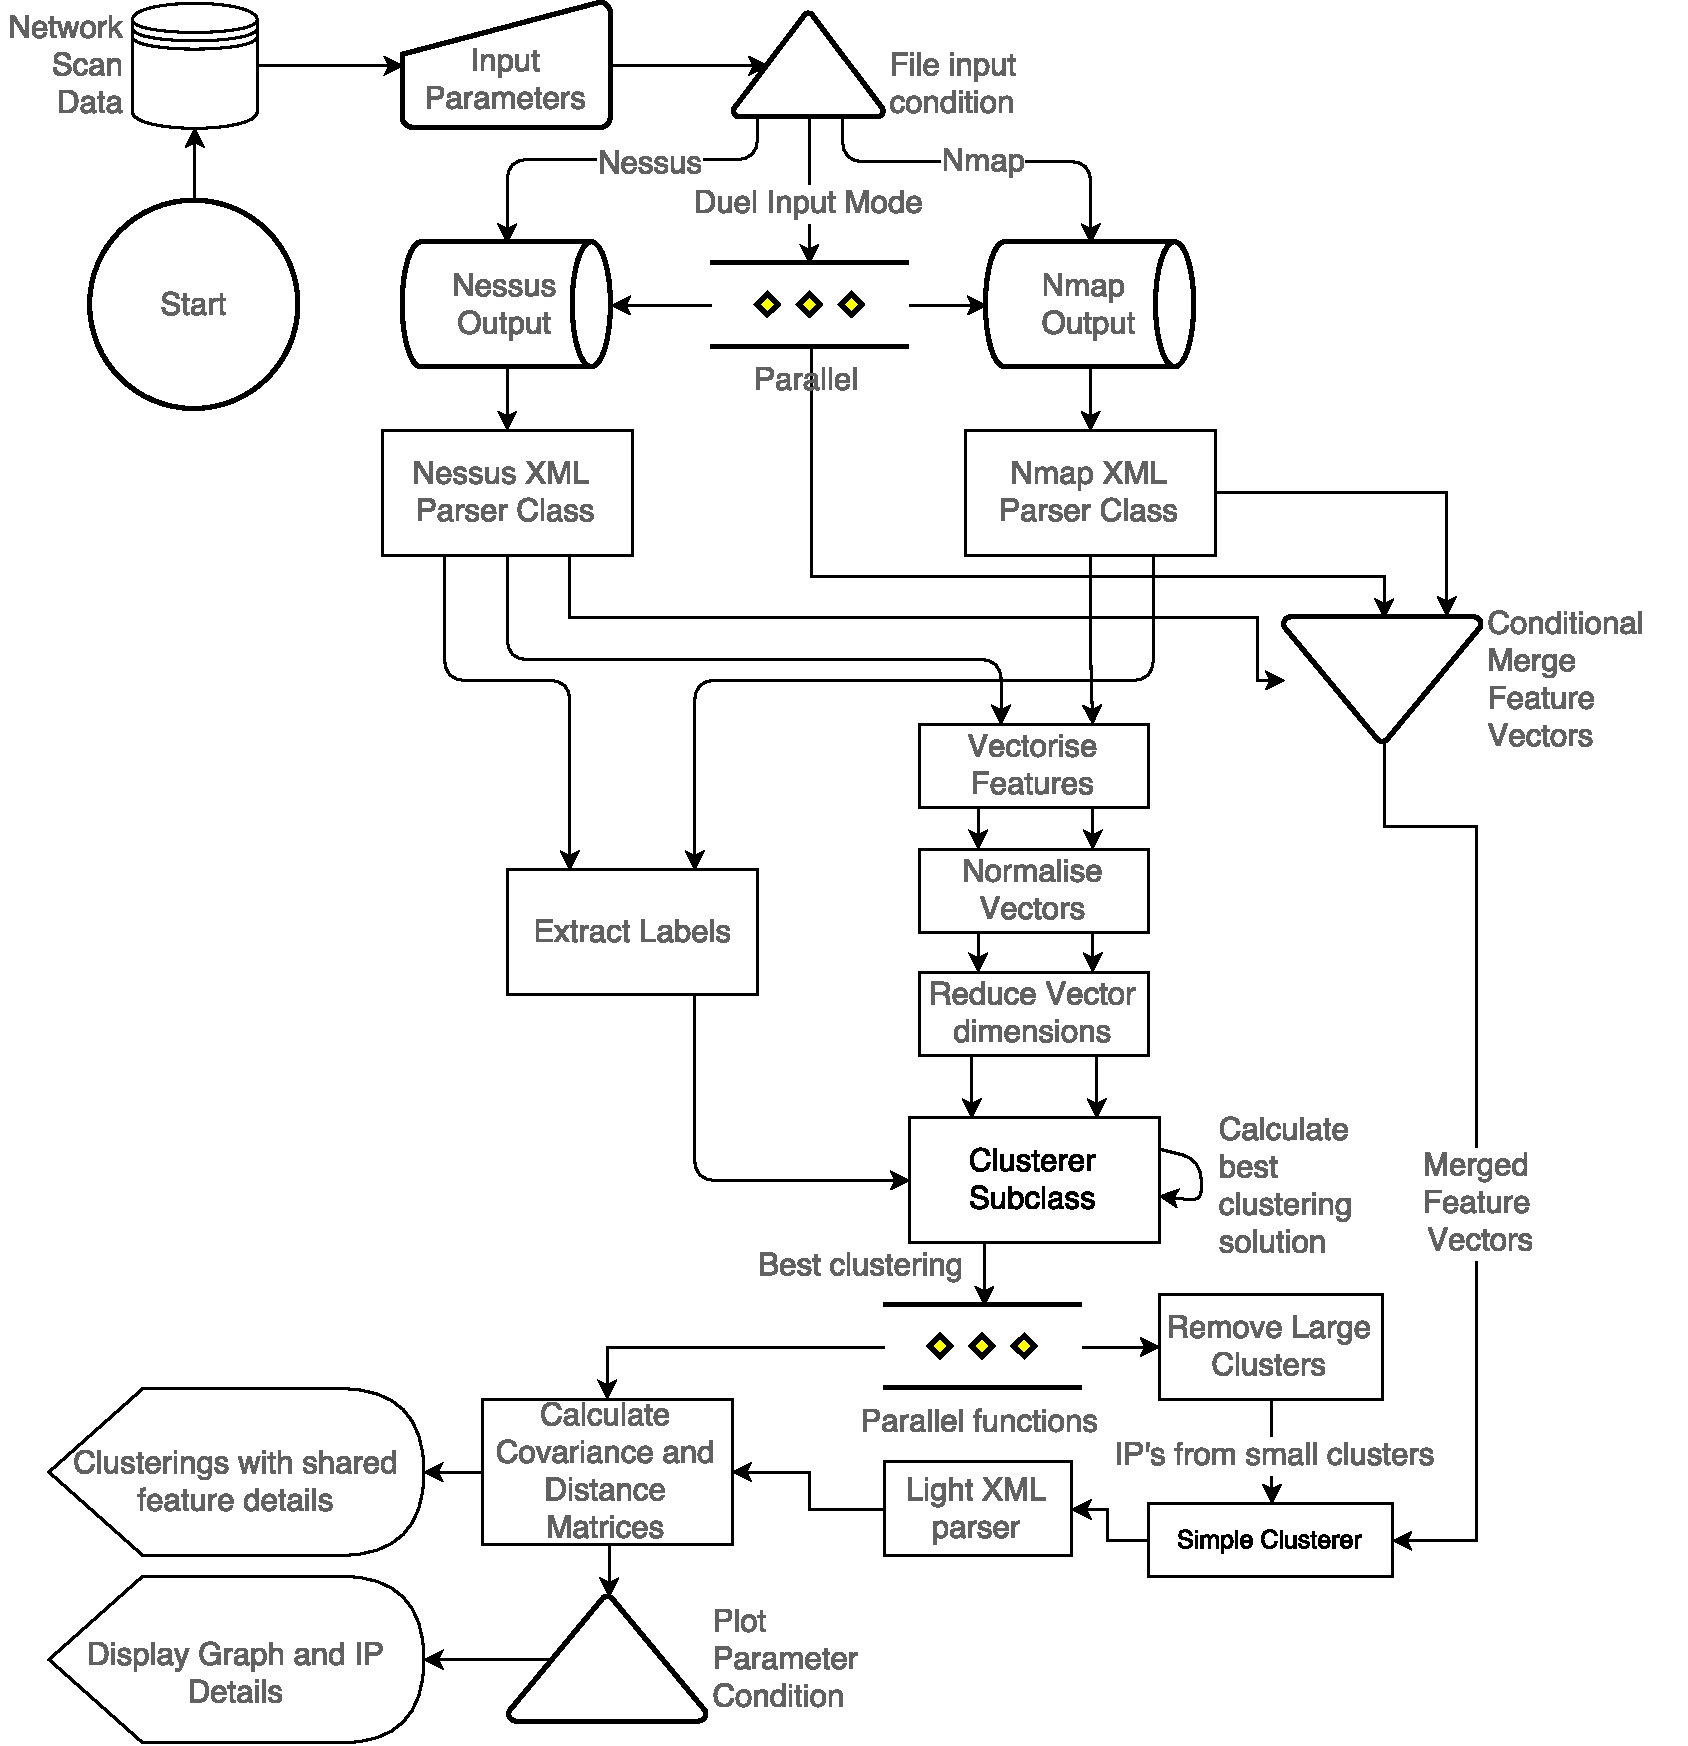
\includegraphics[width=5.5in]{./Figures/flow.pdf}
\caption{Application infrastructure data flow diagram}
\label{flow}
\end{figure}

\paragraph{}Figure \ref{flow} shows the application's primary class infrastructure when in automatic mode. The infrastructure diagram has been created using standard flow diagram symbols to provide understanding of the process types. The application has been programmed for python version 2.7 interpreters and therefore will not have complete functionality without modification for python 3.0 and above. Due to time constraints placed upon this thesis the library NMAP-Cluster, \cite{blackhatnmap}, was used to conserve time.

\paragraph{}In order to execute this application, it is important to have the correct library dependences. This is done via the python package manager ‘PIP' and a requirements file, found in Appendix \ref{requirementsfile}, by executing the command:
\lstset{language=Python}
\begin{lstlisting}
Pip install -r requirements.txt
\end{lstlisting}

\paragraph{}The following sections include detailed descriptions of the processes symbolised within the infrastructure Figure \ref{flow}.  Beginning from the start circle and ending at the display modules.\linebreak

\subsection{Usage and Parameters}
\label{infra1}

\begin{figure}[!h]
\centering
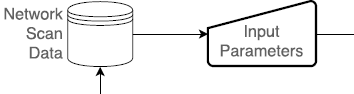
\includegraphics{./Figures/infra1.png}
\caption{Network scan data and input parameter modules from infrastructure diagram at Figure \ref{flow}}
\label{infra1}
\end{figure}

The modules shown in Figure \ref{infra1} are those used to store the network scan data and process the applications input parameters. The Network Scan Data module refers to the XML output of an Nmap scan, Nessus proprietary export file or both. These must be in their respectable formats in order for the parser to recognise them. The files must also be referenced in their correct positional arguments when executing the application such as mentioned in the application usage in Appendix \ref{usage}.

\paragraph{}The Parameters manual input module on Figure \ref{infra1} refers to the parameters that the application requires to select the correct run configuration. This is required because the application has no execution graphical user interface (GUI), the lack of which was decided for several reasons. Such as allowing for scripting, verbose output and terminal pipe operation commands. This type of interface is generally preferred by professionals due to the speed and reliability it provides over a standard GUI. The graphing stage of the application does however, provide a GUI to allow for manipulation of the graphs in multiple ways. The application usage found in Appendix \ref{usage} includes a full description of the possible parameters. The parameters are passed into the data processing section of the application explained in the next session. The three possible run modes are explained in a later section \ref{clustersub}.

\subsection{Data Processing}
\label{infra2}

\begin{figure}[!h]
\centering
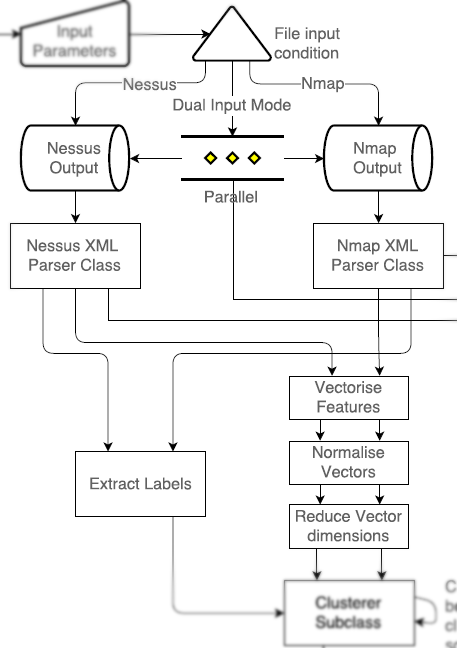
\includegraphics[width=3.5in]{./Figures/infra2.png}
\caption{The data processing section from the infrastructure diagram at Figure \ref{flow} with the irrelevant modules blurred out}
\label{infra2}
\end{figure}
The data processing modules from the infrastructure diagram have been highlighted in Figure \ref{infra2} and will be described in the following paragraphs. \paragraph{}Depending on the files specified within  the input parameters, the application will either feed the Nessus, Nmap or both XML files into the parser classes. These parser classes will take the data from each file and transform it into IP addresses and features which are then passed individually into vectorizers. Vectorization is required for the features to be understood by the clustering algorithm. Vectorization refers to the general process of turning a collection of text (in this case machine attributes) into numerical feature vectors as float values. It is important to note that data from each scanner file is kept separate until the final process. The vectorization class is short and concise due to it having only two purposes, to call the parsers and vectorise the returned results. More information on the vectorization of each file as well as the raw python class code can be found in Appendix \ref{vectorize.py}.

\paragraph{}Once the data has been vectorised it must be normalised in order to avoid large value bias when using dimensionality reduction algorithms such as PCA. Data normalization scales the values to within the same range whilst keeping the data variance and eliminating the bias problem. This is programmed immediately after vectorisation in the applications initialisation class found in its raw code form at Appendix \ref{cluster.py}.

\paragraph{}The major difference between each scanner used is that the Nessus output values include vulnerabilities over Nmap which has superior information on the services and ports of the machine. By using both, the optimal range of information can be achieved, however, this introduces the problem of overfitting which PCA has countered. For more information on PCA refer to dimensionality reduction section \ref{pca} in the introduction. It is possible to greatly modify the output of the two scanners by either using scripts with Nmap or custom plugins for Nessus. Due to the modularity of the application, these modifications to the scanners will not affect the parsers and therefore can be used safely. PCA is also implemented within the initialisation class which can be found in Appendix \ref{cluster.py}. Once PCA is complete, the still separated feature vectors are sent to the clusterer subclass and possibly the conditional merger. The following section will explain the conditional merger of which is represented by symbol in Figure \ref{CMFV}.

\subsection{Small Combined Cluster}
\label{infra3}

\begin{figure}[!h]
\centering
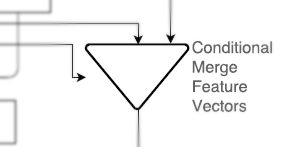
\includegraphics{./Figures/CMFV.png}
\caption{Conditional merge vectors process module from the infrastructure diagram at Figure \ref{flow}}
\label{CMFV}
\end{figure}

\paragraph{}The conditional process of merging the feature vectors, referred to by the symbol in Figure \ref{CMFV}, is executed at this stage, condition dependant on whether dual input mode has been selected when initialising the applications parameters. However, this path must then pause until the main cluster subclass (as represented by the symbol in Figure \ref{clustersub}.) has completed in order to use its clustering outputs. Once this has occurred, each clustering will be duplicated and the large clusters with greater than three IP addresses will be removed from the clustering. This value can be changed based on the network size however the value of three was found to be optimal for networks of size 10 to 1000 from the algorithm tuning stage (this number can be configured for the user's needs by modifying a single variable ‘maxaddresses' within the display class highlighted in Figure \ref{ipno} below). The result of each is combined then re-clustered and the remaining IP's passed through a simpler file parser (compared to that of the ones previously used) to retrieve the information in an un-vectorised text format. This is done to display individual machine information for the end user within the graphing interface. The clustering of these small cluster IP addresses uses the gap statistic (or Elbow method if preferred by user) algorithm to define the numbers of clustered required as appose to user input as these IP's depend on the cluster subclass' algorithm calculated clustering. The main cluster subclass mentioned is explained in the following section \ref{infra4}. Gap statistic and Elbow method formulas can be found in the mathematical model at section \ref{models}.

\begin{figure}[!h]
\centering
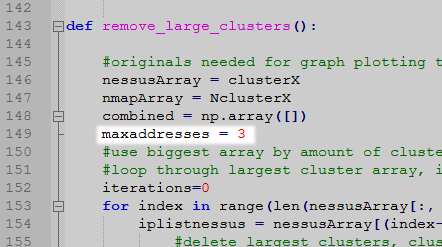
\includegraphics{./Figures/ipno.png}
\caption{Location of the variable which defines the number of maximum IP addresses a cluster is allowed to have for the vulnerability analysis process. The variable is defined within the display.py class's remove large clusters function on line 149}
\label{ipno}
\end{figure}


\subsection{Clustering Algorithm}
\label{infra4}

\begin{figure}[!h]
\centering
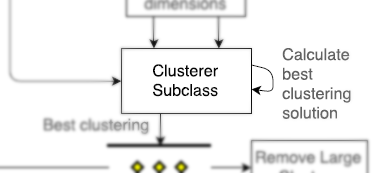
\includegraphics{./Figures/clustersubclass.png}
\caption{Representation of clusterer subclass from infrastructure diagram Figure \ref{flow} spotlighted}
\label{clustersub}
\end{figure}

\paragraph{}The Clusterer subclass represented in the infrastructure diagram by the module in Figure \ref{clustersub}, is where the majority of the calculations are done within the application. This includes the three different modes; manual, assisted and automatic. The raw python code for this module can be found in Appendix \ref{cluster_subclass}. Each mode can be used with a variety of clustering algorithms such as K-means, DBscan and agglomerative clustering. When using dual input mode these functions will execute twice Nessus starting first. A brief summary of each mode is given in the following paragraphs whilst an in-depth algorithm review can be found in section \ref{models}:

    \textbf{Manual:}
     The user supplies all required information to do the clustering. This includes the clustering algorithm and its hyper parameters. If no cluster count ‘K' is provided and K-means was selected, the gap statistic method will be used to calculate the optimal cluster count. An implementation of the elbow method is also included in the application and can be used instead if the gap statistic if the user desires.

    \textbf{Assisted:}
     The user assists the algorithm by suggesting that some samples should or should not be clustered together. This is a much slower process than the other modes but provides the user with complete control over the clustering decisions. The user must specify the clustering algorithm to use from the selection mentioned above when using this mode.

    \textbf{Automatic:}
     Multiple clustering strategies and parameters are used in an attempt to get the best clustering. Unfortunately, this function can only use the K-means clustering algorithm whilst running in dual input mode, due to limitations of the ‘sklearn' library's centroid functions and the time constraints limiting this development as future work. This function goes through each possible iteration of each clustering algorithm up to a maximum cluster value equalling the number of labels in the given dataset. For e.g. in a dataset with ten IP addresses, the maximum allowed clusters is also then. There are multiple selections the user can decide on in terms of which clustering the application will select. This is calculated via a sorting function in the clustering subclass where the user can select between the average silhouette* value, the minimum silhouette* value, the average distance between IP addresses (Euclidian distance by default), the number of clusters in the clustering or the minimum number of common shared features a cluster has in its clustering. These options can also be joined together to make multiple filters. By default, the application uses both the minimum common features and number of overall clusters as filters allowing it to find the clustering with the least number of clusters requiring at least one shared feature. This option is changed near the end of the cluster subclass, changed by uncommenting one line per filter. Each clustering iteration in this loop will calculate the shared positive, negative features, the individual silhouette values and the mean distance to give an overall/per cluster score. Once the iterations are complete for each clustering algorithm the scores and details are used to select one of the clustering's based on the filters and then it is displayed. When using dual input mode, the vulnerability detection on the small clusters explained above in section \ref{CMFV} is continued, due to it requiring these clusters as input. An example of the full text output and graphing interface for the application's automatic mode can be found at Appendix \ref{fictional}.\linebreak
\paragraph{}* The silhouette value is used to validate the consistency of clusters in a clustering by indicating whether there are too many or too few clusters. It provides a value of negative one to positive one indicating how well each IP fits in the cluster.  A high value close to one indicates a good clustering by showing that the IP address is very similar to the other IP addresses in its cluster, whilst being very different to the IP addresses of the neighbouring clusters. Therefore, having a low or negative silhouette value indicates the wrong number of clusters used. The silhouette value has been calculated using the Euclidian distance (described in section \ref{KNN}) within the validation class.
     
\subsection{Covariance and Distance Matrices}
\label{infra5}

\begin{figure}[!h]
\centering
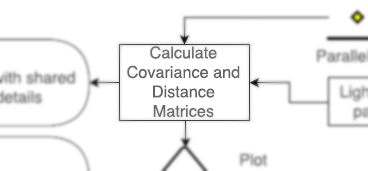
\includegraphics{./Figures/cov.png}
\caption{Representation of covariance and distance matrices function from infrastructure diagram Figure \ref{flow} spotlighted}
\label{cov}
\end{figure}

\paragraph{}Covariance and distance matrices are calculated just before displaying the graphing interface. The function symbol is shown in Figure \ref{cov} above. The output from these functions can be found at the end of the text output, an example is shown in Appendix \ref{exampleoutput}. This is shown for the purpose of giving a technical user greater knowledge of the data-set used which can be interpreted and reported to the client in a security assessment. Specifically, the covariance matrix shows how related the centroids for each clustering are to each other, in other words, their similarity. Covariance will highlight any linear relationships that might be apparent within the dataset with the values ranging from negative one to positive one, high values indicating a positive linear relationship. The Distance matrix shows the literal Euclidian distance between each clustering centroid but by design that also correlates to showing a numericized value defining how different the clusters are from each other. These calculations are done for each clustering result in the current mode (For e.g. three times if using dual mode), however, they are only shown in verbose level one and above modes.

\subsection{Display and Output Modules}
\label{infra6}

\begin{figure}[!h]
\centering
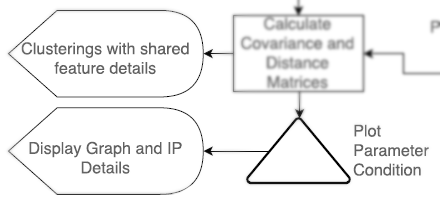
\includegraphics{./Figures/display.png}
\caption{Representation of the display modules from infrastructure diagram Figure \ref{flow} with irrelevant modules blurred out}
\label{display}
\end{figure}

The application will display the main output at the end of its execution as shown in the infrastructure diagram with the symbol from Figure \ref{display}. The application will show a running output as the calculations and cluster iterations are performed, providing that the verbosity level is set to one or higher. The verbosity parameter will only effect the text output and not the graphing interface of the application which will remain identical, an example of full text output using dual mode can be found at \ref{exampleoutput}. Without verbose output selected the text output will only show the cluster details (for both formats if using dual mode). In order for the application to display the graphing interface on clustering class completion the application must be run with the parameter ‘-p' as mentioned in the usage descriptor found in \ref{usage}. The graphs displayed within the graphing GUI are fully manipulatable with zoom, pan and save as functions, however, the graphing interface will differ depending on which mode the application is using. \linebreak
\paragraph{}\textbf{dual mode} graphing interface will display five graphs and a small text segment underneath the bottom graph. The five segments are arranged in a grid of 4 with a large graph beneath the grid spanning both columns as the 5th. The first row of two graphs displays the Nmap output with the right graph solely displaying the centroids and the left displaying the entire Nmap clustering with IP addresses. The second row displays the Nessus graphs in the same configuration as Nmap above. The 3rd row graph displays the IP addresses from the clusters with less than 3 IP addresses (this value is the default and can be changed by following the instruction described in section \ref{CMFV} and Figure \ref{ipno}). The reason for why this is done has been explained within the application brief at section \ref{brief} and the method used explained within section \ref{CMFV}. The text segment beneath the 3rd row graph displays the detected operating system information and the probability of that detection being true. This is shown for each IP address in the small cluster IP addresses graph just above the text segment. An example of the dual mode graphing interface can be found in Figure \ref{example_dual} and Figure \ref{dual}.\linebreak
\paragraph{}\textbf{Standard mode} graphing interfaces are similar to each other as they contain the same two graph split with just different information. The graphs are similar to that of dual mode without the small combined cluster graph of which the left graph includes the full clustering with IP addresses and the right graph solely contains the centroids of those clusters. Two examples of this mode can be found in the Appendix as Figure \ref{split_nessus} for Nessus clustering and Figure \ref{split_nmap} for Nmap clustering, along with the commands used to achieve them. 



\section{Mathematical Model and Theory}
\label{models}

\paragraph{}The following information consists of mathematical representations for the modules in the applications primary class architecture, as shown in figure \ref{flow}.
Parse XML files into matrices V for each input file, consisting of two dimensions' \textit{m} and \textit{n} respectively. The matrices are then vectorised from JSON strings outputted from the parser classes into numerical float representations.
These matrices' data is then normalized using the following formula denoted in the journal of Normalization: A Preprocessing Stage, \cite{normalization}.:
Where Vn is the nth¬ dimension of matrix V and contains the features for each label Vm.
\begin{align*}
{V_n} = \frac{{({V_n} - \;\min \left\{ {{V_n}} \right\})}}{{\left( {\max \left\{ {{V_n}} \right\} - \min \left\{ {{V_n}} \right\}} \right)}}\left( {ne{w_{\max \left\{ {{{\rm{V}}_{\rm{n}}}} \right\}}} - ne{w_{{\rm{min}}\left\{ {{V_n}} \right\}}}} \right) + new\_{\rm{min}}\left\{ {{V_n}} \right\}
\end{align*}

This application will normalise the data to the range of 0 to 1 in which the formula is adjusted to the following:

\begin{align*}
{V_n} = \frac{{({V_n} - \;\min \left\{ {{V_n}} \right\})}}{{\left( {\max \left\{ {{V_n}} \right\} - \min \left\{ {{V_n}} \right\}} \right)}}
\end{align*}

\paragraph{}The Vn dimension of matrix V of each input file is then passed through a principle component analysis formula for dimensionality reduction to two dimensions. This is due to the current number of dimension layers directly correlating to a feature of which there is an average of three hundred per IP address (or \textit{Vm}). This is calculated by using the SKlearn PCA decomposition library which uses the probabilistic model of PCA defined in the journal of Probabilistic Principle Component Analysis, \cite{probabilityPCA}. This algorithm is too complex to be included within the scope of this thesis and therefore is not described here. The result of this PCA algorithm returns a new matrix with two dimensions, which is then used in the K-means clustering algorithm as input with the IP address labels (or \textit{Vm}).

\paragraph{}The standard Lloyd's algorithm for K-means clustering was then used against the PCA output vectors which can be described as the following five stages. This is carried out for each clustering iteration in the cluster class depending on its current mode.

\begin{enumerate}
\item Clusters the Vectors inputs into K number of clusters where K is either assigned manually, iteratively or calculated using the Gap statistic and Elbow values explained below. This depends on the current application mode and user parameters at run time.
\item  Select K number of points at random locations to act as cluster centroids.
\item  Assign objects to their closest plotted centroid per the selected distance function (Euclidian as default).
\item Calculate the new centroid for each cluster in this new clustering.
\item Repeat steps 2, 3 and 4 until the same points are assigned to each cluster in consecutive rounds and no changes are present in the clustering. In the case of automatic mode, the K value will increment up to a maximum equalling the number of IP addresses or labels in Vm.
\end{enumerate}

\paragraph{}However, the user can also select the use of DBscan or Agglomerative clustering algorithms instead of K-means for any mode apart from dual input. However, due to the limited usage they provide for the applications design goals, will not be described in this thesis. 

\paragraph{}Each clustering result of this algorithm has several calculations carried out upon it in order to validate and provide scores to the clustering. These calculations are denoted in section \ref{clustersub}. The primary function used to score these clustering's is a silhouette value which has been defined in the journal, Silhouettes: A graphical aid to the interpretation and validation of cluster analysis, \cite{silhouette}. A full description of what this value provides for the user is included at the end of section \ref{clustersub}. The formulas used to calculate the silhouette value are taken from the previously mentioned journal and are described below.

\paragraph{}For each vector \textit{i}, \textit{a(i)} would be the average dissimilarity of vector \textit{i} with all other vectors within the same cluster. \textit{b(i)} is the lowest average dissimilarity of vector \textit{i} to any other cluster of which vector \textit{i} is not a member of. The cluster with the lowest value for \textit{b(i)} is the closest neighbouring cluster and therefore the most similar. This defines the following formula for silhouette value \textit{s(i)}.\linebreak
\begin{align*}
s\left( i \right) = \frac{{b\left( i \right) - a\left( i \right)}}{{\max \left\{ {a\left( i \right),b\left( i \right)} \right\}}}
\end{align*}

\paragraph{}The resulting clustering's are sorted based on the filters mentioned in \ref{clustersub} and the best clustering is chosen. This best clustering is passed through into the small combined cluster algorithm described in section \ref{CMFV} as well as the display class in \ref{display}.

\paragraph{}When the application uses the K-means clustering algorithm and a value for K is not defined, the application will attempt to calculate the optimal value for K via either the Gap Statistic or Elbow value methods depending on the user's preferences. This is changed within the optimal k means class with the default value being the Gap Statistic method. The python implementation of the Gap Statistic method can be found in the Appendix \ref{gapstatistic} with the formulas used were originally developed by Stanford researchers from the journal, Estimating the number of clusters in a data set via the gap statistic, \cite{gapref}. The implementation of the researchers' algorithm within this application can be described by the following points.

\begin{enumerate}

\item Cluster the data via K-means from the range of k=1 to k=max and calculate the variance quantity variable \textit{Wk} (primarily used for elbow method).
\item Generate the reference data sets \textit{B} and cluster them with the same k values as previous step. 
\item Calculate the gap statistic value with the following formula: \linebreak
\begin{align*}
Gap\left( k \right) = \left( {\frac{1}{B}} \right)\mathop \sum \limits_{b = 1}^B logW_{kb}^* - log{W_k}.
\end{align*}
\item Calculate the standard deviation using: \linebreak
\begin{align*}
sd\left( k \right) = {\left[ {\left( {\frac{1}{B}} \right)\mathop \sum \limits_b (logW_{kb}^* - {{(\left( {\frac{1}{B}} \right)\mathop \sum \limits_b logW_{kb}^*)}^2}} \right]^{1/2}}
\end{align*}
\item Then define ${s_k} = \;\sqrt {1 + \frac{1}{B}} sd\left( k \right)$ which allows the optimal number of K to be the smallest k such that $Gap\left( k \right) \ge Gap\left( {k + 1} \right) - {s_{k + 1}}$. 

\end{enumerate}

The Covariance and distance matrices displayed prior to graphing output are calculated using the following methods. More information on these values can be found in \ref{infra5}.
Covariance for a given centroid vector dimensions \textit{x} and \textit{y} is calculated using the formula: 
\begin{align*}
cov\left( {x,y} \right) = \frac{{(\mathop \sum \nolimits_{i = 1}^n \left( {{x_i} - \bar x} \right)\left( {{y_i} - \bar y} \right))\;}}{{n - 1}}
\end{align*}

This is calculated for each centroid in the chosen clustering and displayed in a matrix.
The distance matrix displays the Euclidian distance between the x and y values for each centroid in the clustering.

\section{Application Testing}
\label{testing}
\paragraph{}Unfortunately due to the sensitive nature of the data required by the application, there are no datasets to be found publicly available online. Therefore, in order to design a proof of concept test procedure a dataset must be created using a significant network size to simulate the proportions of a real organizational network. The size requirements of this dataset limit the use of virtualized machine networks due the raw processing power required for a network of that size, hence, the permission was granted to allow for the scanning of a private network laboratory in the University of Abertay. The laboratory consisted of approximately 50 online devices at the time of scanning. The raw scan output files for Nmap and Nessus can be found within the thesis' artefacts, hacklab analysis folder with the file names hacklab\_new.xml and hacklab\_new.nessus respectfully.

\paragraph{}The creation of this dataset required installing the Nmap and Nessus scanner tools on a separate device plugged into the network for this sole purpose. The device used to enter the network and execute the scans was a Dell latitude E6410 laptop running the latest rolling release kernel of Arch Linux. This setup was used specifically to replicate a similar scenario to that of what an industry professional might encounter. The latest stable releases of the required software were used. At the time of writing this thesis (April 2017) those reference numbers were as follows: 
\begin{itemize}
\item Nmap 7.40
\item Nessus 6.10.5 
\item Python 2.7.13
\item Python Libraries
\begin{itemize}
\item backports-abc==0.4
\item bokeh==0.12.1
\item certifi==2016.8.8
\item cycler==0.10.0
\item futures==3.0.5
\item Jinja2==2.8
\item MarkupSafe==0.23
\item matplotlib==1.5.1
\item numpy==1.11.1
\item pyparsing==2.1.8
\item python-dateutil==2.5.3
\item pytz==2016.6.1
\item PyYAML==3.11
\item requests==2.11.0
\item scikit-learn==0.17.1
\item scipy==0.18.0
\item singledispatch==3.4.0.3
\item six==1.10.0
\item tornado==4.4.1
\item tabulate==0.7.7
\end{itemize}
\end{itemize}

The Nmap scan was created using the following command: 
\begin{lstlisting}[language=python]
nmap -A -O -oX hacklab.xml 10.0.0.0/24
\end{lstlisting}
The -Ox flag in this command exports the scan as an XML which is the only export format the clustering application currently supports.\linebreak
The Nessus scan was created by using the default scan policy in the advanced scan mode with the same scope as nmap, 10.0.0.0/24. This was then exported as the latest version of the proprietary Nessus XML format from the scan overview page.

\paragraph{}Once both scans have completed the next step is to remove the testing device used from the XML files manually due to each scanner retrieving greatly differing results from the testing machine compared to other machines on the network. This step is crucial and ignoring it will manipulate the final result of the clustering algorithm rendering it inaccurate. The artefact files have had this step done prior to submission.

The scan files have then been passed through the clustering application using the following commands for each input type in automatic mode:\linebreak

\textbf{Nmap}
\begin{lstlisting}[language=bash]
cluster.py -s automatic -vv -p "../hacklab analyses/hacklab_new.xml"
\end{lstlisting}

\textbf{Nessus}
\begin{lstlisting}[language=bash]
cluster.py -s automatic -vv -p -N "../hacklab analyses/hacklab_new.nessus"
\end{lstlisting}


\textbf{Dual Input}
\begin{lstlisting}[language=bash]
cluster.py -s automatic -vv -p -t -N -tp "../hacklab analyses/hacklab_new.xml" "../hacklab analyses/hacklab_new.nessus"
\end{lstlisting}

\paragraph{}More information and the results for this proof of concept test can be found in Appendix section \ref{hacklab}. These results will be validated within the thesis conclusions.



%%Chapter
\chapter{Results}
\label{chap:chapter1}

%paragraph with reference in bibligraphy.bib
\paragraph{}This paragraph provides a reference to Einstein's paper: \cite{Einstein}. The paragraph also contains an inline equation $a+b=c$.

%Section
\section{Section}
\label{sec:section1}

\paragraph{}This paragraph is located in Chapter~\ref{chap:chapter1} and talks about Figure~\ref{fig:sampleFigureLabel}.

%Figure
\begin{figure}[h]
\centering
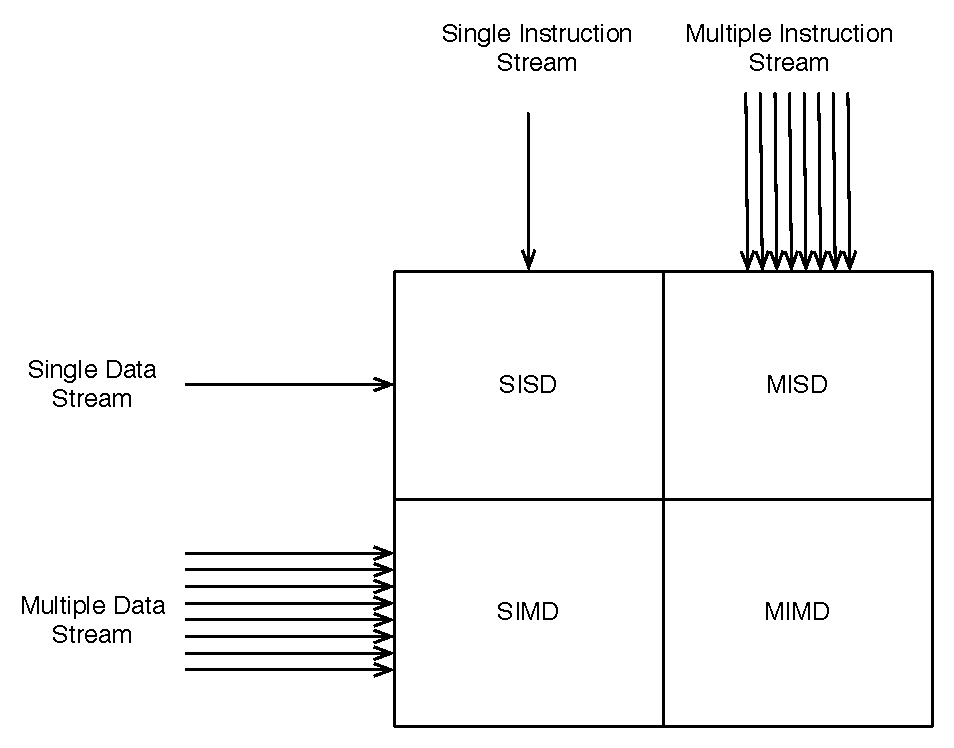
\includegraphics[width=3.5in]{./Figures/sampleFigureFlynn.pdf}
\caption{sample figure caption}
\label{fig:sampleFigureLabel}
\end{figure}

%Subsection
\subsection{Subsection} 
\label{ssec:subsection1}


\paragraph{}This is a paragraph located in a subsection.  This paragraph also reference a  Figure~\ref{fig:sampleFigureLabel}.


%subsection 2
\subsection{Subsection}
\label{ssec:subsection2}

\paragraph{}This paragraph reference another subsection~\ref{sec:section1}.
%% !TEX root=dissertationmain.tex
%Chapter
\chapter{Discussion and Results}
\label{discussion}

\paragraph{}In this chapter, the application developed and the thesis as a whole will be reviewed. 
\paragraph{}The aim of this dissertation was to design and develop a proof of concept tool to be utilised by the red teaming individuals such as penetration testers during a security assessment. The application was required to be versatile, portable and reliable allowing it to be used in any size of network topology. From the Application Brief \ref{brief}, the application serves as an additional tool to be used during the initial enumeration stage of a penetration test. It will provide the user with several graphs and statistics on the network which are not provided by currently available commercial tools, such as a visual network overview of machine differences. The application primarily targets are security professionals and network administrators whom want a visual representation of their overall network security due to how well the application scales to network sizes.
\paragraph{}The main findings of this thesis show that red teaming can benefit greatly from machine learning techniques and more research needs to be carried out to move the industry forward towards more accurate, faster and efficient software tools. The results from the proof of concept testing of the application against a network with approximately fifty hosts can be found at Appendix \ref{hacklab} and information on how the test was carried out can be found in section \ref{testing}. The results show that the application was successful in classifying the difference and vulnerability level of the hosts on the network. The following paragraphs will analyse the results in order to show how this conclusion was achieved.
\paragraph{}The application relies on the two scan files used, Nmap and Nessus, for its accuracy as they provide the bases of all the information used for every calculation involved in the software. This means that these two scan files can be used to validate the application results by manually checking each scanner output within their respective applications. \linebreak
\paragraph{}First, the results of the application must be outlined and analysed to then be compared against the files, this is carried out in the following subsection.
\subsection{Test Results Analysis and Validation}
\label{testresults}

\paragraph{}This subsection will summarise the results of the application testing followed by the validation and in depth explanation of those results.

\subsubsection{Analysis of Results}
\label{results_analysis}
\paragraph{}The application detected the five IP addresses in Figure \ref{ips} as the most vulnerable based on their vulnerabilities and properties. This is shown in both the application's GUI output in Figure \ref{results} and its text output in \ref{hacklabtext}: 

\begin{figure}
\label{ips}
\begin{center}
\begin{tabular}{ |c| }
\hline
10.0.0.1\\ \hline
10.0.0.185\\ \hline
10.0.0.3\\ \hline
10.0.0.5\\ \hline
10.0.0.7\\ \hline
\end{tabular}
\end{center}
\caption{The five detected vulnerable IP addresses from the Hacklab Analysis testing section in \ref{testing}}
\end{figure}


\begin{figure}[!h]
\centering
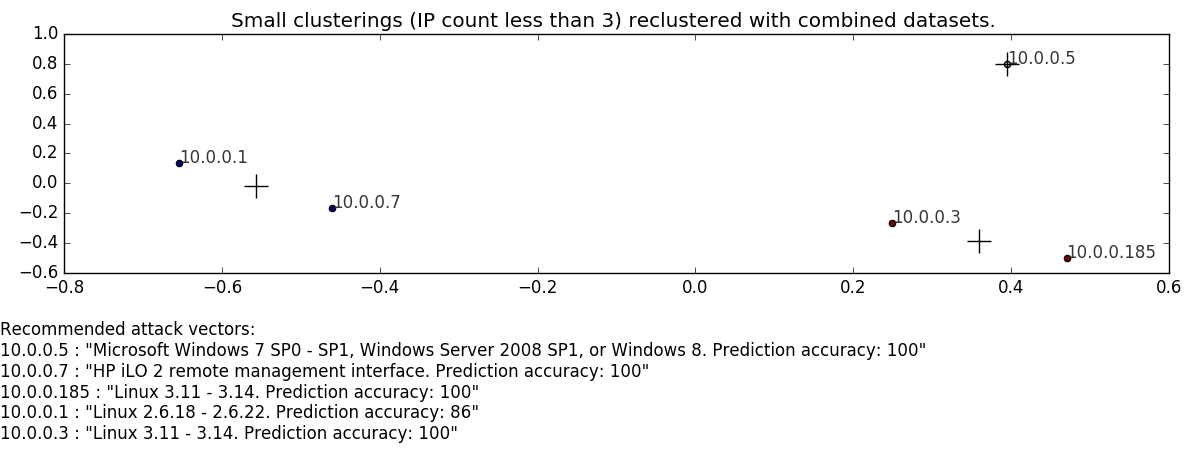
\includegraphics[width=6in]{./Figures/results.png}
\caption{Short excerpt from the application's graphing output in automatic dual mode from Abertay University's Hacklab network analysis \ref{testing}}
\label{results}
\end{figure}

\paragraph{}Figure \ref{results} shows the lower segment of the full results in Figure \ref{dual}, specifically, the vulnerability clustering section of the application explained in \ref{CMFV}. The top graph represents the IP addresses from the small clusters, in this case clusters with less than three IP addresses, clustered via how similar they are to each other and their vulnerability properties, if any were detected by the Nessus scanner. This means that these hosts have the greatest difference from the majority of others in the network and most likely have known vulnerabilities. However, if the majority of hosts on the network have the same vulnerability, then the application will only display the \textit{different} ones, resulting in those hosts not being shown. This scenario is discussed further on in the discussion. 

\paragraph{}From the application's maximum verbosity text output in \ref{hacklabtext}, line 237 shows that the five selected hosts were selected based on 491 different features per host, which was achieved by joining both feature sets together for this part of the application. The features are passed through PCA, similarly to that of the regular clustering section of the application to reduce these 495 features into a two-dimensional dataset. The split for this feature set in this particular test was 288 for Nessus (line 7) and 203 for Nmap (line 11), this relates to a 59\% bias in the clustering towards the Nessus parsed features. Due to Nessus providing all the information about the vulnerabilities and Nmap providing a greater overall amount of system information, the two sets of data work together to give the application a more complete overview of the network. The Nessus bias allows the application to prioritise the vulnerabilities in the clustering algorithm over general system information. However, this ratio is fluid and changes depending on the Nessus configuration used and the networked hosts themselves. This unequal ratio is due to the fact that, while the Nmap scanner returns the same amount of data per machine without variance, the Nessus scanner outputs vary greatly depending on the number and detail of the vulnerabilities detected. This means that a network with a greater number of detailed vulnerabilities on its hosts will provide a much greater clustering bias towards the Nessus data, rather than the Nmap data. This bias only occurs when both data-sets are combined during the final vulnerability detection stage of the application explained in \ref{CMFV} and not during individual tool clustering's. Based off this information, the application recommends these afore mentioned five hosts to be targeted first during a manual security assessment as they will provide the greatest chance of success.

\paragraph{}The text information beneath the graph in Figure \ref{results} shows the operating systems detected for each host in \ref{ips} as well as the probability percentage of this prediction being accurate. The four graphs in figure \ref{results2} represent the other half of the applications output in automatic dual mode. Each graph is titled to show the user what they each represent. As mentioned previously these clustering's use their respectable tool files and thus, do not contain the bias that Figure \ref{results} has. Two of these four graphs are the exact same as those found if the application were to execute using the single dataset mode for each tool as such demonstrated in Figures \ref{split_nessus} and \ref{split_nmap}. This section of the output can be found explained in section \ref{display}. The IP addresses of hosts in Figure \ref{ips} can be seen within the two clustering's, showing how those hosts relate to the other hosts of larger clusters, in the same terms as Figure \ref{results} but keeping the tool output features to their individual graphs.

\begin{figure}[!h]
\centering
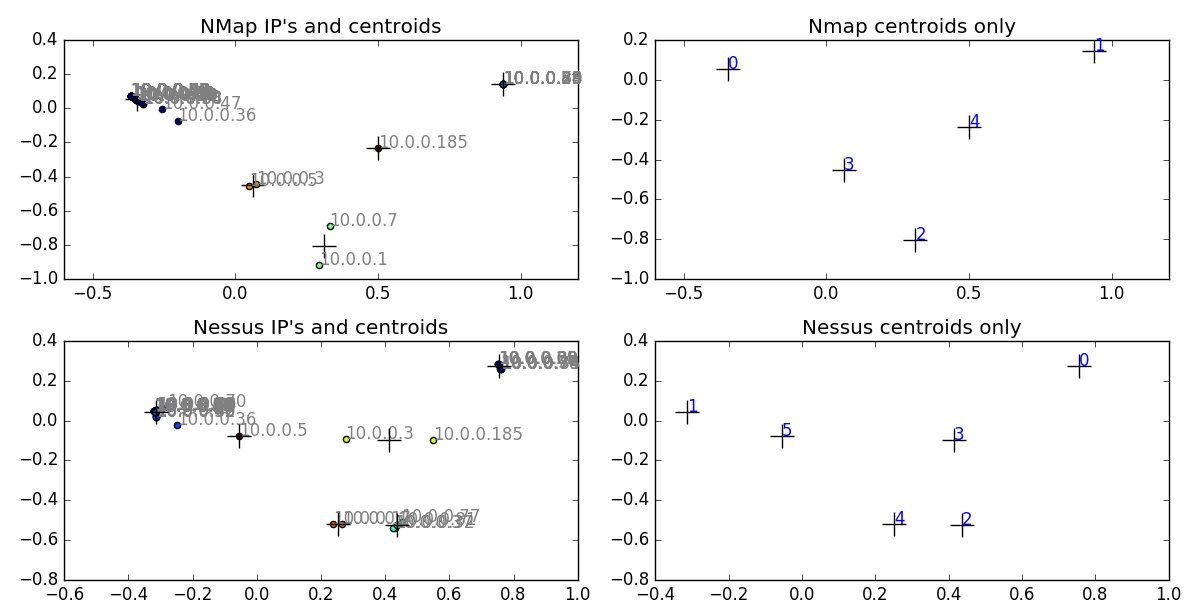
\includegraphics[width=6in]{./Figures/results2.png}
\caption{standard tool output graphs from application's graphing output in automatic dual mode from Abertay University's Hacklab network analysis \ref{testing}}
\label{results2}
\end{figure}

\subsubsection{Validation}

\paragraph{}In order to determine whether the detected IP addresses in Figure \ref{ips} are that of the most differential hosts, each tool output must be investigated individually. By uploading the Nessus file onto a Nessus web interface of version 6 or above, it is possible to see an overview of the file with colour coded bars for each host. This is represented in Appendix Figures \ref{hacklab_nessus1} and \ref{hacklab_nessus2}. The original image was split into two Figures simply due to the size being too large for this paper. The key for the colour coded bars in the Nessus overview is as follows:
\begin{center}
\begin{tabular}{ |c|c| }
\hline
Red & Critical rank vulnerability\\ \hline
Yellow & Medium rank vulnerability\\ \hline
Green & Low rank vulnerability\\ \hline
Blue & Host information\\ \hline
\end{tabular}
\end{center}

\paragraph{}Through analysis of the Nessus overview using the key above, the differences in vulnerabilities per host are made apparent as visually intended by the developer, Tenable\textsuperscript{TM}. By specifically viewing the selected hosts in this overview, it can be observed that \textbf{they are indeed, the most unique compared to the other hosts} in terms of Critical, Medium and Low ranked vulnerabilities. When using this method to compare hosts, it is important to not provide as much weight to the key colour blue representing the host information as to the vulnerability codes. This is because the blue host information is given much lower importance than the vulnerabilities in the Nessus parser class. If the keys shown above were weighted equally, the clustering would not have the bias towards the vulnerabilities and result in a less accurate prediction by the algorithm. Unfortunately, there is no similar visualisation method to validate the Nmap graph and requires manually reading the output XML file and comparing It to the application graphs.

\paragraph{}Another method to validate the network is a manual approach, which requires in-depth prior knowledge of the network used. This approach is possible for individuals such as network administrators who might use this tool for the purpose of confirming the results of a security assessment, and not to discover new information. This approach is not possible for scenarios such as capture the flag events where there is no prior knowledge of the network and its hosts. The manual approach involves comparing the application's verbose text output, such as each cluster's shared features, to the individual's prior knowledge of the network. The following section will give a critical evaluation of the application.

\subsection{Critical Evaluation}
\label{criteval}
\paragraph{}This section will provide a short critical evaluation of the application and its performance in its intended role.

\paragraph{}As previously mentioned in this discussion, if the used network contains a large number of hosts with the same vulnerability, then those hosts become the majority and since the application, in its essence, finds the differences in hosts, the clustering might not reflect the hosts with that vulnerability accurately. This problem is difficult to solve completely as it would involve changing the application's core design architecture. A possible untested solution however, is as follows. By adding a new layer on top of the parser classes to make it aware of common vulnerabilities in the dataset, then displaying them to the user directly would mitigate this problem. Another possible workaround is simply for the user to manually check for any common, major vulnerabilities within the Nessus overview as mentioned in the previous section and take them into account when considering the application's results.

\paragraph{}Unfortunately, due to the nature of the datasets used including sensitive information, there are no online datasets that the application could use. This makes the creation of a proper testing procedure difficult as all data used for this application within this project was created specifically for this project. This means that the application is to be taken simply as a proof of concept and not a finalised design.

\paragraph{}Due to project time constraints, the primary automatic dual mode of the application was only able to be implemented with the K-means algorithm however, both DBscan and agglomerative implementations are already fully programmed and integrated into the model. The only issue stopping these algorithms to be integrated into this mode is the fact the sklearn python library (used to calculate several of the clustering functions) does not include centroid support for them and one would have to be manually programmed, which would take more time than was available for the project. Once that feature has been implemented, the two algorithms can be re-enabled with minimal difficulty.

\paragraph{}The application has been optimised for model prediction accuracy over performance times, however, each class module within the application has been programmed modularly allowing for the easy modification by others without prior knowledge of how it was created. Variables may be changed easily, such as the IP cut off limit for the vulnerability detection stage explained in \ref{CMFV} without fear of it causing problems elsewhere in the application. Another such example of modularity is allowing the option of modifying the parsing classes to change what it taken as features and labels from each tool output. When using a network with less than a hundred hosts such as that of in the testing chapter, the application will take between one and three minutes to complete on the dual automatic mode. Other modes such as manual and assisted can be completed in less than thirty seconds. This performance could be improved by converting parts of the application models to a language such as C++ although this would greatly reduce the customization level of the application, which is one of the primary design features. Upon successful completion of the clusterer, the application will write to two files. One of which is a dot file including the primary clustering and the other is a target file including the selected hosts from the results. The latter file can be imported into many tools such as Metasploit and Armitage to manually assess those hosts. The former can be imported into graphing tools such as Gephi to interface with them in a different manner than the integrated interface. Both these output files can be easily disabled they are not needed by modifying one line at the end of the initialization class.

\subsection{Discussion Summary}
\paragraph{}The findings in this thesis contribute towards developing a machine learning arsenal of tools that can be used by security professionals, as well as help balance the research in the security industry by providing a unique red teaming proof of concept tool. The results of the testing are of direct practical relevance to the red team, and such align with the design goals highlighted in \ref{brief}. Only a couple of other studies, to our knowledge, have examined the use of machine learning in red teaming. It is clear that further research in this area is necessary before machine learning can become common place in this industry sector, however, this paper has helped cleared ground for this research to take place in. This paragraph marks the end of the discussion and the following section will provide conclusions to the paper.

%% !TEX root=dissertationmain.tex
\chapter{Conclusions and Recommendations}
\label{conc}

\paragraph{}This chapter will summarize the thesis, provide future development recommendations and describe its impact on the field of machine learning for offensive security.

\paragraph{}The machine learning field of study is continually evolving with deep learning being at the forefront of the field, providing levels of accuracy and efficiency previously unobtainable due to the lack of available processing power. This paper uses classification algorithms including, but not limited to, K-means clustering with silhouette and gap statistic values, as well as data statistic calculations such as covariance matrices. There has been much research carried out for machine learning in the blue team field, however, as highlighted in the literature review \ref{litreview}, there have been \textit{very few} research papers dedicated to red teaming or offensive security. The primary goal of this thesis was to improve this balance by creating grounds for more research and development on the red team side of security, as well as develop an application tool for example usage in this field. This goal was achieved as described via the following paragraphs.

\paragraph{}This thesis documents the design, development and testing of a proof of concept red teaming application, written in Python. The application, in brief, uses machine learning and common network scanning tools to provide the user with advanced information about a network. The application's primary function is to apply clustering techniques on the data from Nmap (open source tool) and Nessus (developed by Tenable\textsuperscript{TM}) scanner outputs (both together or individually) in several different approaches, determining vulnerable hosts on the network, based on probability and feature similarity. The application includes manual, assisted and automatic modes for each type of tool input, then provides results in both text and, if selected, graphical format. The application is very versatile and, by design, can be completely configured to adapt to any type of network environment using several parameters from \ref{usage}.  An example of the resulting output from the application during the testing stage can be found in \ref{hacklab}. These results include in depth information about each cluster as well as graphs displaying the clusterings. The application is able to determine possible vulnerable hosts based on several factors described in \ref{CMFV}, with a bias towards the Nessus vulnerabilities analysed in \ref{results_analysis}. As a tool designed for security professionals, does not include a graphical user interface, it is instead configured and executed through a single command. Subsequently to execution, the application writes two files to its local directory as follows. A dot file consisting of the primary clustering to allow it to be imported into other commercial graphing applications such as Gephi. Along with a text file consisting of the targets from the vulnerability analysis, which can be imported into exploitation tools such as Metasploit Framework from Offensive Security\textsuperscript{\textregistered} and Hydra, a cracking suite developed by THC.

\paragraph{}There is however, an issue in determining the vulnerabilities, which occurs when the application uses data from hosts with a majority encompassing the same vulnerability. In this case the resulting output of the combined function in dual mode will not show these hosts based off that specific vulnerability, in other words, it is possible that the application would not depend on that vulnerability for analysis. This is due the clustering algorithm by design, as it detects and highlights the differences in the hosts then displays the most different of them all in extra to the full clusterings. This issue and solutions have been discussed and analysed in \ref{criteval}. This can be resolved through future work, however, more future work recommendations based on this thesis are as follows.

\paragraph{}The application machine learning model may be reprogrammed to utilise neural networks or other advanced machine learning algorithms as appose to K-means to classify each host. This would increase the predictability and efficiency of the model although, careful considerations to the variety in network configurations as well as the computational power impact should be taken into account if this approach is used. An intuitive graphical user interface may be implemented on top of the application, which would benefit users with less confidence in the current command line interface. Currently the application returns the probability of the operating system detection due to time constraints, however, it would be more beneficial for the end user if the application returned the pre-detected vulnerabilities for each host as well as the chances of their existence on the live system. The current modular python implementation approach allows for easy modification of the core modules by technical users depending on the desired use, this has the unfortunate side effect of slow execution times due to the Python interpreter.  The application can be ported to other lower level languages such as C++ instead, allowing for a much faster execution time in exchange for lower customisability. Support for more network scanners may be implemented without much more development by adding extra parser classes and modifying the display class. This would make increase reliability and usability of the application in the case where the current scanners are too noisy or obstructive to be used on a certain network. Due to the proof of concept nature of the application in its current state, in addition to the improvements previously mentioned, further testing and polishing may be carried out to release the application for use in the field depending on its applied license agreement.

\paragraph{}In conclusion, this thesis has created grounds for further research and development into machine learning for offensive security by proving its effectiveness in the field. This thesis has also provided several examples for further development based on the internally developed application. 


%now enable appendix numbering format and include any appendices
\appendix
\chapter{Appendix stuff}

\paragraph{}Lorem ipsum dolor sit amet, consectetur adipiscing elit, sed do eiusmod tempor incididunt ut labore et dolore magna aliqua. Ut enim ad minim veniam, quis nostrud exercitation ullamco laboris nisi ut aliquip ex ea commodo consequat. Duis aute irure dolor in reprehenderit in voluptate velit esse cillum dolore eu fugiat nulla pariatur. Excepteur sint occaecat cupidatat non proident, sunt in culpa qui officia deserunt mollit anim id est laborum.


%uncomment next line to change bibliography name to references
%\renewcommand{\bibname}{References}
\bibliography{bibliography}        %use a bibtex bibliography file refs.bib
\bibliographystyle{agsm}  %use the plain bibliography style

\end{document}

